93. \begin{figure}[ht!]
\center{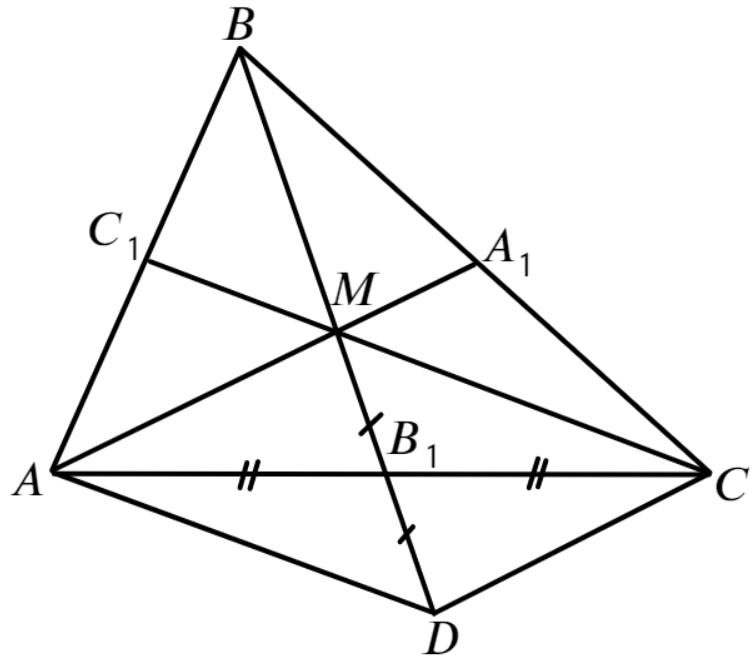
\includegraphics[scale=0.35]{g9-92.png}}
\end{figure}\\
Продолжим $MB_1$ так, чтобы $MB_1=B_1D.$ Тогда в четырёхугольнике $AMCD$ диагонали делятся точкой пересечения пополам, а значит он является параллелограммом и $CD=AM.$ Так как медианы делятся точкой пересечения $M$ в отношении $2:1,$ считая от вершины, стороны треугольника $CMD$ равны $8,\ 10$ и $14.$ Найдём его площадь по формуле Герона: $p=\cfrac{8+10+14}{2}=16,\ S=\sqrt{16\cdot8\cdot6\cdot2}=16\sqrt{6}.$ Тогда $S_{AMCD}=2S_{\Delta CMD}=32\sqrt{6},\ S_{\Delta AMC}=\cfrac{1}{2}S_{ABCD}=16\sqrt{6}.$ Так как медианы делят любой треугольник на 6 равновеликих, $S_{\Delta ABC}=3S_{\Delta AMC}=48\sqrt{6}.$\newpage\noindent
